% Experimental Setup
%==============
In this section, experiments are performed to evaluate the performance
of the framework on the real-world datasets collected from New York
City (NYC). In particular, the aim is to answer the following questions:
\begin{itemize}
    \item \textbf{Q1}: How does the framework perform as compared to the state-of-the-art techniques in predicting crime occurences of different categories?
    \item \textbf{Q2:}  Does the framework consistently outperform other baselines in terms of prediction accuracy \emph{w.r.t} different time windows with different training and testing time periods?
    \item \textbf{Q3:} How is the performance of the framework variants with different combinations of key components in the joint framework?
    \item \textbf{Q4:} How the different choices of model parameters (e.g., embedding size and number of hidden layers) affect the performance of the framework?
    \item \textbf{Q5:} How is the interpretation of the framework in capturing the unknown temporal relevance when predicting crimes?
\end{itemize}

\section{Experimental Setup}
\subsection{Data}
The framework was evaluated with three datasets collected in New York City (NYC): (Detailed in Table \ref{table:dataset}).

1) \textbf{Crime Data}: The framework was valuated on the
real-world crime data collected from New York City (NYC) Open-Data portal from Jan 1, 2014 to Dec 31, 2014. Each crime record
is in the format of (crime category, latitude, longitude, timestamp).
In this work, the focus is on the crime categories whose average frequency of occurrence is greater than 9 times for each region in
a city per month, namely, \textit{Robbery, Burglary, Felony Assault} and
\textit{Grand Larceny}.
\begin{table}
\centering
\begin{tabular}{l|c|c|c|c|c|c|}
\toprule
\textbf{Data Source} &\multicolumn{6}{|c}{\textbf{New York City Crime Reports}}\\[0.1cm]
\hline
\hline
Time Span &\multicolumn{6}{|c}{From Jan, 2014 to Dec, 2014}  \\[0.1cm]
\hline
Category &\multicolumn{3}{|c|}{Burglary}  &\multicolumn{3}{|c}{Robbery}\\[0.1cm]
\hline
Number of Instances &\multicolumn{3}{|c|}{16,720} &\multicolumn{3}{|c}{16,557}\\[0.1cm]
\hline
Category &\multicolumn{3}{|c|}{Felony Assault}  &\multicolumn{3}{|c}{Grand Larceny}\\[0.1cm]
\hline  
Number of Instances &\multicolumn{3}{|c|}{19,059} &\multicolumn{3}{|c}{51,577}\\[0.1cm]


\toprule
\textbf{Data Source} &\multicolumn{6}{|c}{\textbf{Point-of-Interests (POI)}}\\[0.1cm]
\hline
\hline
Category &\multicolumn{2}{|c|}{\#} & \multicolumn{2}{|c|}{Category} &\multicolumn{2}{|c}{\#}    \\[0.1cm]
\hline
Arts \& Entertainment &\multicolumn{2}{|c|}{720} & \multicolumn{2}{|c|}{Automotive \& Vehicles} &\multicolumn{2}{|c}{1505}    \\[0.1cm]
\hline
Business to Business &\multicolumn{2}{|c|}{3717} & \multicolumn{2}{|c|}{Computers \& Technology} &\multicolumn{2}{|c}{637}    \\[0.1cm]
\hline
Education &\multicolumn{2}{|c|}{1062} & \multicolumn{2}{|c|}{Food \& Dining} &\multicolumn{2}{|c}{3385}    \\[0.1cm]
\hline
Government \& Community &\multicolumn{2}{|c|}{3116} & \multicolumn{2}{|c|}{Health \& Beauty} &\multicolumn{2}{|c}{4336}    \\[0.1cm]
\hline
Home \& Family &\multicolumn{2}{|c|}{3616} & \multicolumn{2}{|c|}{Legal \& Finance} &\multicolumn{2}{|c}{1782}    \\[0.1cm]
\hline
Real Estate \& Construction &\multicolumn{2}{|c|}{4675} & \multicolumn{2}{|c|}{Shopping} &\multicolumn{2}{|c}{1874}    \\[0.1cm]
\hline
Sports \& Recreation &\multicolumn{2}{|c|}{384} & \multicolumn{2}{|c|}{Others} &\multicolumn{2}{|c}{1378}    \\[0.1cm]
\hline


\toprule
\textbf{Data Source} &\multicolumn{6}{|c}{\textbf{311 Public-Service Complaints}}\\[0.1cm]
\hline
\hline
Time Span &\multicolumn{6}{|c}{From Jan, 2014 to Dec, 2014}  \\[0.1cm]
\hline
Category &\multicolumn{3}{|c|}{Noise}  &\multicolumn{3}{|c}{Blocked Driveway}\\[0.1cm]
\hline
Number of Instances &\multicolumn{3}{|c|}{151,174} &\multicolumn{3}{|c}{92,335}\\[0.1cm]
\hline
Category &\multicolumn{3}{|c|}{Illegal Parking}  &\multicolumn{3}{|c}{Building Use}\\[0.1cm]
\hline  
Number of Instances &\multicolumn{3}{|c|}{69,100} &\multicolumn{3}{|c}{27,724}\\[0.1cm]
\bottomrule

\end{tabular}
\vspace{0.2cm}
\caption{Detail of the datasets}
\label{table:dataset}
\end{table}

Figure \ref{fig:img2} shows the geographical distributions of different categories of crime occurrences in New York City (NYC) on August
and December, respectively. From these visualization results, it
can be observed that (i) different geographical regions have different
crime occurrence distributions given a specific crime category; (ii)
crimes of different categories exhibit different occurrence patterns
in the same region of a city; (iii) crimes from different time periods
show different geographical distribution patterns. Inspired by the
above observations, the inherent correlations between regions, crime categories and time slots with an attention-based hierarchical recurrent networks is explicitly explored.
\begin{figure}[t]
\captionsetup[subfigure]{font=scriptsize,labelfont=scriptsize}
\centering
\begin{subfigure}{0.24\textwidth}
\centering
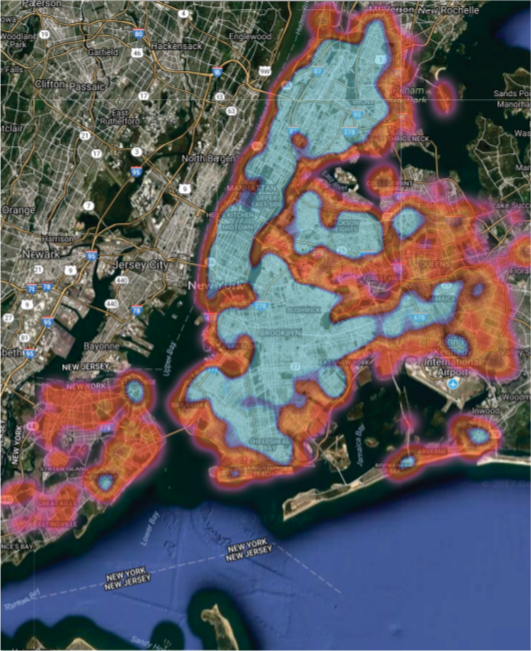
\includegraphics[width=0.9\linewidth]{Chapter5/Images/burglary.png} 
\caption{Burglary – Aug}
\label{fig:subim1}
\end{subfigure}
\begin{subfigure}{0.24\textwidth}
\centering
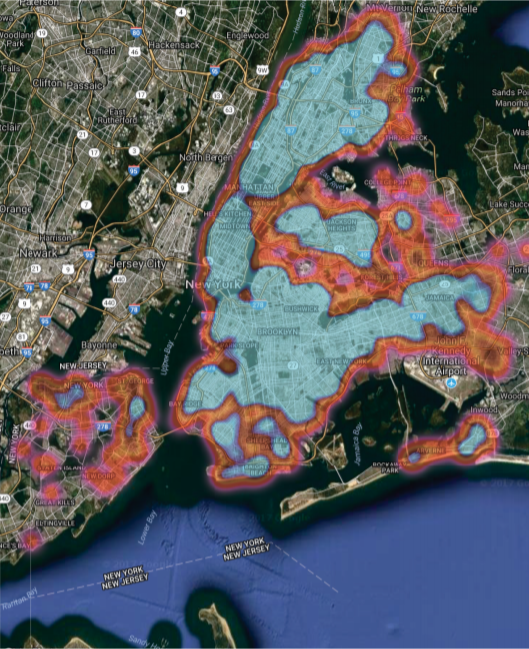
\includegraphics[width=0.9\linewidth]{Chapter5/Images/robbery.png}
\caption{Robbery – Aug}
\label{fig:subim2}
\end{subfigure}
\begin{subfigure}{0.24\textwidth}
\centering
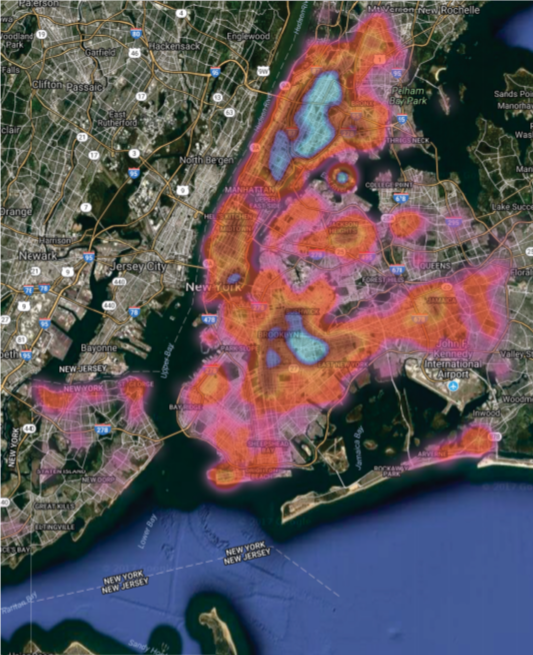
\includegraphics[width=0.9\linewidth]{Chapter5/Images/felony.png}
\caption{Felony – Aug}
\label{fig:subim3}
\end{subfigure}
\begin{subfigure}{0.24\textwidth}
\centering
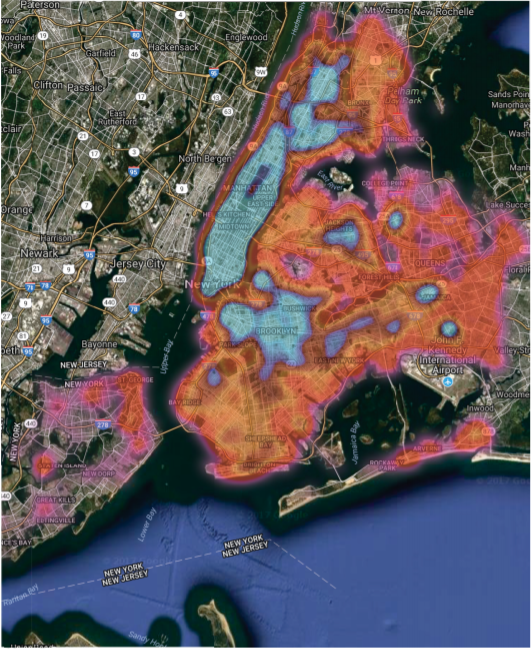
\includegraphics[width=0.9\linewidth]{Chapter5/Images/grand.png}
\caption{Grand – Aug}
\label{fig:subim4}
\end{subfigure}
 
\caption{Geographical distribution of crime occurrences with different categories in New York City on August and December,
respectively.}
\label{fig:img2}
\end{figure}

2) \textbf{Point of Interests (POIs)}: 24,031 POIs of 14
categories (\emph{e.g.,} Arts \& Entertainment and Shopping, detailed in
Table 1) were collected. Each POI is formatted as (venue name, category, address, latitude, longitude).

3) \textbf{311 Public Service Complaint Data}: These datasets are collected from 311 Service which documents urban complaint reports
of different categories from citizens through a mobile app or phone
calls. Each complaint record is in the format of (complaint category,
latitude, longitude, timestamp).4 key complaint categories (\emph{e.g.,} Noise, Blocked Driveway, Illegal Parking and Building
Use) were selected which are studied in [33].
New York City was divided into 77 disjointed geographical regions based on the information of political districts 2. Each region
is an area of the city as defined for police purposes.

\subsection{Parameter Settings}

The hyper-parameters play important roles in the framework, as they determine how the model will be
trained. In the experiments, each of the key parameters
in the framework are varied and others are fixed to examine the parameter sensitivity
of the proposed method. The framework is implemented based
on TensorFlow and Adam [17] is used as the optimizer to learn the
model parameters. The hyperparameter settings are optimized with
the grid search strategy. In the experiments, the batch size is set
as 64, learning rate as 0.001 and and the number of hidden layers in
Multilayer Perceptron component as 3.

\subsection{Baselines}

The framework is compared with the following four
types of baselines: (i) variant of Recurrent Neural Network models for time series prediction. (\emph{i.e.,} GRU); (ii) conventional time
series forecasting methods (\emph{i.e.,} ARIMA and SVR); (iii) both the
conventional and neural feature-based supervised learning methods for classification (\emph{i.e.,} LR, MLP and Wide\&Deep); (iii) tenor
factorization-based method for predictive analytics (\emph{i.e.,} TriMine).
\newpage
\begin{itemize}
    \item \textbf{Support Vector Regression (SVR)} [3]: a non-parametric machine learning method for regression based on kernel functions.
    
    \item \textbf{Auto-Regressive Integrated Moving Average (ARIMA)} [16]: a well-known time series prediction model for understanding
    and predicting future values in a time series.
    
    \item \textbf{Logistic Regression (LR)} [13]:  a statistical model which forecasts a region’s crime occurrence based on temporal features
    (\emph{e.g.,} the day of a week and the month of a year) extracted from
    historical crime logs.
    
    \item \textbf{Multilayer Perceptron (MLP)} [7]: it incorporates temporal features from historical distributions of crimes into a deep neural
    network architecture, to model the non-linearities in crime data.
    
    \item \textbf{Tensor Decomposition (TriMine)} [24]: this method is applied
    to predict crime occurrences by extending the Matrix Factorization scheme to consider the temporal dimension of crime data.
    Specifically, a three-dimension tensor is utilized to represent the
    crime series of all regions in a city ($1^{st}$ dimension–region, $2^{nd}$
    dimension–crime category and $3^{rd}$ dimension–time).
    
    \item \textbf{Wide and Deep Learning (Wide\&Deep)} [4]:  a wide \& deep
    learning framework to combine the strengths of wide linear
    models and deep neural networks for predictive analytics.
    
    \item \textbf{Gated Recurrent Unit (GRU)} [5]:  a gating recurrent neural network model which has fewer parameters than LSTM by lacking
    an output gate to achieve computational efficiency.
\end{itemize}
In the experiments, all parameters are also learned using the Adam
optimizer.

\subsection{Evaluation Protocols}

To validate the performance of all
compared methods in predicting crime occurrences (posed as a
classification problem) of each region in a city, two types of
evaluation metrics are adopted: (i) \emph{F1-score} (trade-off between precision
and recall) is used to evaluate the accuracy of predicting a specific category
of crime occurrence. (ii) \emph{Marco-F1} and \emph{Micro-F1} [12] is used to
evaluate the prediction accuracy across different crime categories.
These metrics have been widely used in the problems of multi-class
classification to calculate the overall performance across different
classes. In this work, each crime category (\emph{e.g.,} burglary
and robbery) is considered as an individual class. Note that a higher Micro-F1
and Macro-F1 score indicates better performance.

In the evaluation, the datasets are split chronologically into
training (6.5 months), validation (0.5 month) and test (1 month)
sets. The validation datasets are used to tune hyper-parameters and
test datasets are used to evaluate the performance of all compared algorithms. All experiments are conducted across 30 consecutive
days in test time frames and the average performance is reported.

\section{Performance Validation (Q1 and Q2)}

To investigate the performance of all compared methods on different
targeted time frames, evaluation results from Nov 2014
and Dec 2014 are shown. The following key observations can be made.\\
(1) Table \ref{table:macro} and Table \ref{table:category} list the evaluation results of all compared
methods with respect to different training and test time windows.
It can be observed that the proposed framework outperforms other baselines over different time frames (i.e., from Nov and Dec).In addition, although different time windows reflect a
spectrum of temporal diversity which is maintained by month and
season variation, the proposed method consistently achieves the best
performance by capturing this temporal dynamic. Therefore, the
evaluation results across different time frames demonstrate the effectiveness of the framework in modeling time-evolving dependencies
in crime sequences and reasonably interprets the importance of
past crime occurrences in predicting future crimes


\begin{table}[htb]
\centering

\begin{tabular}{c|c|c|c|c}
\toprule
Month
 &\multicolumn{2}{|c|}{August}
&
\multicolumn{2}{|c}{September}\\[0.1cm]
\hline
% \\\cmidrule(r){1-2} \cmidrule(r){2-3}\cmidrule(l){4-5}
Algorithm & Macro-F1 & Micro-F1    & Macro-F1 & Micro-F1 \\[0.1cm]
% \cmidrule(r){1-1} \cmidrule(r){2-2} \cmidrule(r){3-3}
\hline
SVR & 0.6312 & 0.5400 & 0.6394 & 0.5457\\[0.1cm]
ARIMA & 0.6281 & 0.5478 & 0.6269 & 0.5451\\[0.1cm]
LR & 0.6260 & 0.5199 & 0.6307 & 0.5248\\[0.1cm]
MLP & 0.6389 & 0.5317 & 0.6407 & 0.5317\\[0.1cm]
TriMine & 0.6434 & 0.5538 & 0.6402 & 0.5335\\[0.1cm]
Wide\&Deep & 0.6326 & 0.5366 & 0.6431 & 0.5464\\[0.1cm]
GRU & 0.6316 & 0.5659 & 0.6354 & 0.5720\\[0.1cm]
\toprule
Proposed framework & \textbf{0.6657} & \textbf{0.6009} & \textbf{0.6683} & \textbf{0.6110}\\
\bottomrule
\end{tabular}

\vspace{0.2cm}
\begin{tabular}{c|c|c|c|c}
\toprule
Month
 &\multicolumn{2}{|c|}{October}
&
\multicolumn{2}{|c}{November}\\[0.1cm]
\hline
% \\\cmidrule(r){1-2} \cmidrule(r){2-3}\cmidrule(l){4-5}
Algorithm & Macro-F1 & Micro-F1    & Macro-F1 & Micro-F1 \\[0.1cm]
% \cmidrule(r){1-1} \cmidrule(r){2-2} \cmidrule(r){3-3}
\hline
SVR & 0.6312 & 0.5400 & 0.6394 & 0.5457\\[0.1cm]
ARIMA & 0.6281 & 0.5478 & 0.6269 & 0.5451\\[0.1cm]
LR & 0.6260 & 0.5199 & 0.6307 & 0.5248\\[0.1cm]
MLP & 0.6389 & 0.5317 & 0.6407 & 0.5317\\[0.1cm]
TriMine & 0.6434 & 0.5538 & 0.6402 & 0.5335\\[0.1cm]
Wide\&Deep & 0.6326 & 0.5366 & 0.6431 & 0.5464\\[0.1cm]
GRU & 0.6316 & 0.5659 & 0.6354 & 0.5720\\[0.1cm]
\toprule
Proposed framework & \textbf{0.6657} & \textbf{0.6009} & \textbf{0.6683} & \textbf{0.6110}\\
\bottomrule
\end{tabular}

\vspace{0.2cm}

\begin{tabular}{c|c|c}
\toprule
Month
&
\multicolumn{2}{|c}{December}\\[0.1cm]
\hline
% \\\cmidrule(r){1-2} \cmidrule(r){2-3}\cmidrule(l){4-5}
Algorithm & Macro-F1 & Micro-F1 \\[0.1cm]
% \cmidrule(r){1-1} \cmidrule(r){2-2} \cmidrule(r){3-3}
\hline
SVR & 0.6394 & 0.5457\\[0.1cm]
ARIMA & 0.6269 & 0.5451\\[0.1cm]
LR & 0.6307 & 0.5248\\[0.1cm]
MLP & 0.6407 & 0.5317\\[0.1cm]
TriMine & 0.6402 & 0.5335\\[0.1cm]
Wide\&Deep & 0.6431 & 0.5464\\[0.1cm]
GRU & 0.6354 & 0.5720\\[0.1cm]
\toprule
Proposed framework & \textbf{0.6683} & \textbf{0.6110}\\
\bottomrule
\end{tabular}
\vspace{0.2cm}
\caption{Crime prediction results across different categories in terms of Macro-F1 and Micro-F1}
\label{table:macro}
\end{table}


\begin{table}
\centering
\begin{tabular}{c|c|c|c|c}
\toprule
Category
 &\multicolumn{2}{|c|}{Burglary}
&
\multicolumn{2}{|c}{Robbery}\\[0.1cm]
\hline
% \\\cmidrule(r){1-2} \cmidrule(r){2-3}\cmidrule(l){4-5}
Algorithm & November & December    & November & December \\[0.1cm]
% \cmidrule(r){1-1} \cmidrule(r){2-2} \cmidrule(r){3-3}
\hline
SVR & 0.4896 & 0.5241 & 0.5201 & 0.5367\\[0.1cm]
ARIMA & 0.4850 & 0.5234 & 0.5333 & 0.5441\\[0.1cm]
LR & 0.5032 & 0.5246 & 0.5032 & 0.5246\\[0.1cm]
MLP & 0.5087 & 0.5633 & 0.5483 & 0.5537\\[0.1cm]
TriMine & 0.5276 & 0.5306 & 0.5161 & 0.5576 \\[0.1cm]
Wide\&Mine & 0.4985 & 0.5482 & 0.5325 & 0.5549\\[0.1cm]
GRU & 0.5147 & 0.5378 & 0.5491 & 0.5684 \\[0.1cm]
\toprule
Proposed framework & \bf0.5902 & \bf0.5912 & \bf0.5993 & \bf0.6228\\
\bottomrule
\toprule
Category
 &\multicolumn{2}{|c|}{Felony Assault}
&
\multicolumn{2}{|c}{Grand Larceny}\\[0.1cm]
\hline
% \\\cmidrule(r){1-2} \cmidrule(r){2-3}\cmidrule(l){4-5}
Algorithm & November & December    & November & December \\[0.1cm]
% \cmidrule(r){1-1} \cmidrule(r){2-2} \cmidrule(r){3-3}
\hline
SVR & 0.5842 & 0.5893 & 0.8426 & 0.8354\\[0.1cm]
ARIMA & 0.5821 & 0.5627 & 0.8366 & 0.8301\\[0.1cm]
LR & 0.5704 & 0.5512 & 0.8440 & 0.8405\\[0.1cm]
MLP & 0.5961 & 0.5600 & 0.8432 & 0.8423\\[0.1cm]
TriMine & 0.6144 & 0.5913 & 0.8442 & 0.8415 \\[0.1cm]
Wide\&Mine & 0.5743 & 0.5675 & 0.8430 & 0.8436 \\[0.1cm]
GRU & 0.6316 & 0.5659 & 0.5815 & 0.5561 \\[0.1cm]
\toprule
Proposed framework & \textbf{0.6246} & \textbf{0.6120} & \textbf{0.8443} & \textbf{0.8432}\\
\bottomrule
\end{tabular}
\vspace{0.2cm}
\caption{Crime prediction results for individual category in terms of F1-score}
\label{table:category}
\end{table}
